\chapter{Introduction to 5G and Key Technologies}
\label{chapter2}
The rapid advancement in the wireless communications shows the huge success in the wireless communication system. The advancement started with second generation (2G) system's debut in 1991 which were commercially launched on the GSM standard in Finland by Radiolinja. 2G systems were significantly more spectrally efficient compared to their predecessors and 2G also introduced the data services for mobile starting with SMS text messages, picture messages and multimedia messages (MMS). From 2G we migrated to 3G system which were first launched in 2001 and had fast mobile Internet access. 3G also introduced video calls and mobile TV and was able to provide information transfer speed of at least 2 Mbit/s. The 4G wireless systems were designed to be fully based on IP telephony where all the voice communications and multimedia sessions are delivered over Internet protocol (IP) networks~\cite{4561570}. 4G systems use orthogonal frequency division multiplexing (OFDM), multiple-input multiple-output (MIMO), and link adaptation technologies for a long term evolution (LTE) radio interface. 4G wireless networks can support data rates of up to 1 Gb/s for low mobility and up to 100 Mb/s for high mobility scenarios. The next evolution in wireless mobile communications is the fifth generation (5G) which is expected to be deployed by 2020.

Due to a sharp increase in number of wireless mobile devices and the shortage of the wireless spectrum, researchers have started to investigate 5G wireless technologies. It is expected that the 5G network will achieve 1000 times the system capacity, 10 times the spectral efficiency, energy efficiency, data rate and 25 times the average cell throughput. This translates to a peak data rate of 10 Gb/s for low mobility and peak data rate of 1 Gb/s for high mobility scenarios. The table~\ref{tableG} below shows the comparison between 2G, 3G, 4G and 5G cellular communication system. 

\begin{table*}[!ht]
\centering
\label{tableG}
\caption{Cellular Technologies Comparison between different generations of deployed digital cellular networks. Data rates, standard and implementation technology is compared for the 3G, 4G and 5G}
\resizebox{\textwidth}{!}{\begin{tabular}{c c c}
\textbf{3G} & \textbf{4G} & \textbf{5G} \\\hline
1990/2002 & 2000/2010 & 2010/2022 \\\hline
2 Mbps & 200 Mbps -- 1 Gbps (low mobility) & 10 Gbps and higher (low mobility) \\\hline
WCDMA, CDMA-2000 & Unified Long Term Evolution (LTE) standard & In-progress \\\hline
\end{tabular}}
\end{table*}

\section{5G Cellular Architecture}
\label{5gcell}
The base station density is increasing drastically due to the huge spike in the use of heterogeneous networks to support massive exchange of information over the air. The heterogeneous networks are already standardized in 4G but the architecture is not natively designed to support them. The huge network densification requires major changes in the cellular architecture of 5G communication system. Wireless users mostly stay indoors for about 80\% of the time, while only 20\% of the mobile users stay outdoors~\cite{4623708}. The conventional cellular architecture consists of an outdoor base station in the middle of a cell communicating with mobile users irrespective of the user's location. Since the signal incur a large penetration loss since it has through go through buildings, thus restricting the data rates, spectral and energy efficiency of the wireless transmissions. The key idea behind 5G cellular communication is to separate the outdoor and indoor scenarios so that the penetration loss and shadowing caused by buildings can be avoided. This will be achieved by using distributed antenna system (DAS) and massive MIMO technology (also referred to as ''Large-Scale Antenna Systems'') where spatially located antenna arrays with hundreds of antenna elements are deployed. Using large number of antenna arrays in base station renders the channels to the different devices quasi-orthogonal and very simple spatial multiplexing procedures quasi-optimal. The favorable action of the law of large numbers smoothens out frequency dependencies in the channel and thus leads to huge gains in the spectral efficiency~\cite{Boccardi2014}. The BSs deployed outdoors will be equipped with massive MIMO distributed around the cell and connected to the BS via optical fibers as a backbone network. The outdoor mobile users are normally equipped with very limited number of antenna elements, but the devices can form a virtual massive MIMO links to increase the capacity and spectral efficiency. The Figure~\ref{5garch} shows the proposed heterogeneous 5G cellular architecture by C. Weng, et.al~\cite{Wang2014}. 
 
\begin{figure}[!ht]
	\centering
\includegraphics[width=\textwidth,height=10cm,keepaspectratio]{images/Gill/5G/5gsystemarch.eps}
	\caption{5G Architecture}
	\label{5garch}
\end{figure}

The proposed 5G cellular architecture consists of macrocells, microcells, small cells and relays. In this type of network, mobile users can be offloaded to nearby femto base stations instead of all competing for macro cells to increase the data rates per user. The massive MIMOs will be depoloyed outside of the buildings and will be connected to the wireless access points inside the building via cables for indoor users. The initial startup cost for the 5G infrastructure will be very high but it will vastly improve the cell througput, spectral efficiency and data rate of the cellular system in the long run. By separating the cellular architecture into indoor and outdoor scenarios, with indoor users only requiring to communicate with indoor wireless access points many technologies can be utilized for short-range communications with massive data rates. The examples of short-range communications system include high speed Wi-Fi, ultra wideband (UWB) , mm-wave communications (3--300 GHz)~\cite{6515173} and visible light communications (VLC) (400--490 THz)~\cite{4212879}. The backbone networks of 5G will move from copper and fiber to mm-wave wireless connections enhancing cooperation and connectivity between base stations. It is worth noting that mm-Wave and light communication systems use higher frequencies not traditionally used for cellular technologies. Using mm-Wave frequencies currently saturated radio spectrum band from 700 MHz to 2.6 GHz can also be augmented for wireless communications. The 28 GHz and 60 GHz bands are currently available with spectrum allocations of over 1 GHz of band-width. Originally intended for Local Multipoint Distribution Service (LMDS) use in the late 1990's, these licensees could be used for mobile cellular as well as backhaul~\cite{502029}. These sub tera-hertz frequency waves do not penetrate solid building walls very well and can readily be absorbed or scattered by gases, rain, and foliage. The path-loss at 60 GHz at 1m distance is around 68 dB and at 10 m distance path-loss is 88 dB. Therefore, it is hard to use these waves for outdoor and long distance applications. However, with large bandwidths available, mm-Wave and visible light communication technologies can greatly increase the transmission data rate for indoor scenarios. Besides using mm-Wave and VLC, dynamic spectrum access (DSA) can also be utilized to solve the spectrum scarcity problem. The important characteristics of DSA systems is their ability to exploit knowledge of their spectral environment to adapt and modify their operational parameters to efficiently access the spectrum~\cite{4211144}. The key promises of these systems are that they open up the possibility of highly flexible and efficient management and reuse of spectrum across all its dimensions. The cognitive radio~\cite{819467}, build on software-defined radio is the intelligent, adaptive and frequency agile wireless devices that will underlie most forms of future DSA systems. In this thesis, we have implemented the cooperative spectrum sensing using software-defined radios which are utilizing the spatial gain to improve the accuracy of primary user detection. The primary user detection is very important factor in utilizing the spectrum efficiently so we don't interfere with the incumbent users. The heterogeneous networks has already been introduced in 4G LTE architecture but their use has been very limited and but due to rapid densification  of wireless devices 5G cellular architecture should be a heterogeneous one. In the following sections we will discuss the some key technologies which will drive the advancement of 5G cellular system.

\section{Key Technologies of 5G System}

To understand the engineering challenges facing 5G cellular communication, it is paramount to first identify its requirements. The following items are requirements in each key dimension, but it is important to note that all of these need to be satisfied simultaneously to achieve bounds set for 5G technology. Due to the rapid advancement in IoT devices different applications will place different requirements on the performance of the network. Applications with high data rate for e.g., streaming high-definition videos may have relaxed latency and quality of service (QoS) requirements compared to driverless cars or public safety applications, where latency QoS are paramount but lower data rates can be tolerated. Before we get into the key features of 5G cellular system, we first need to classify the impact of new technologies and their implications for 5G. These new technologies are classified leveraging the Henderson-Clark model and are as follows~\cite{Boccardi20140}:
\begin{itemize}
\item New changes are required at both the node and architectural level, for e.g. the introduction of codebooks and signaling support for a large number of antennas (Massive-MIMO).

\item Complex changes in the design of network nodes are required, for e.g. introduction of new waveforms. These are the modifications required at the component level.

\item The heterogeneous architecture of 4G system will act as a good benchmark for future 5G systems, but we need disruptive changes in the 5G system architecture. 

\item To achieve data rates in the order of tens of gigabits with much lower latency cannot be achieved by merely building on the current system architecture, we need to completely redesign the system at node and component level. 
\end{itemize}

Some key features for the 5G wireless system which we think will be important in revolutionizing the cellular radios for the massively dense wireless devices in the future.

\subsection{Massive MIMO}

Massive (Very Large) multiple-input multiple-output MIMO Systems is a multiple antenna technology which is becoming ready for wireless communications and has been implemented for wireless broadband standards like LTE and Wi-fi. The key idea behind using large number of antennas is to create more possible signal paths and to achieve better performance in terms of data rate and link reliability via spatial multiplexing~\cite{massivemimo}. Figure~\ref{massivemimo} describes the implementation of massive MIMO technology using the patch antenna arrays communicating with several user equipments (UE). The implementation is proposed for the 5G system as the patch antenna arrays can be mounted on the walls of the buildings due to their thin size and can provide high-speed data rate coverage in outdoor environment also. 

\begin{figure}[!ht]
	\centering
\includegraphics[width=\textwidth,keepaspectratio]{images/Gill/5G/beams.eps}
	\caption{Massive-MIMO implementation using patch antenna arrays}
	\label{massivemimo}
\end{figure}

Massive-MIMO is the key technology for 5G cellular system and it has a clear distinction from the existing LTE/4G system through the use of a very large number of service antenna that can operate adaptively and in a fully coherent manner. It proposes utilizing a very high number of antennas to multiplex data signals for several UEs on each time-frequency resource, focusing the beam toward the intended directions while minimizing intra- and inter-cell interference. Using hundreds and thousands of antennas help in focusing the beam in a smaller regions of space, thus bringing huge improvements in throughput, gain and energy efficiency. This can particularly help in bringing large improvement when combined with simultaneous scheduling of a large number of UEs. Figure~\ref{beamforming} shows the beamforming using $N$ = 4,8,12 and 16 antenna elements using linear dipole arrays. The antenna array gain for $N = 4,~8,~12,~16$ is 9.23 dB, 12.3 dB, 14.1 dB and 16.15 dB respectively. By using hundred or thousands of antenna array element we can achieve a very high gain and throughput. Massive MIMO may require major architectural changes, particularly in the design of macro base stations, and it may also lead to new types of deployments. 

\begin{figure}[!h]
\centering
  \subfloat[$N$ = 4]{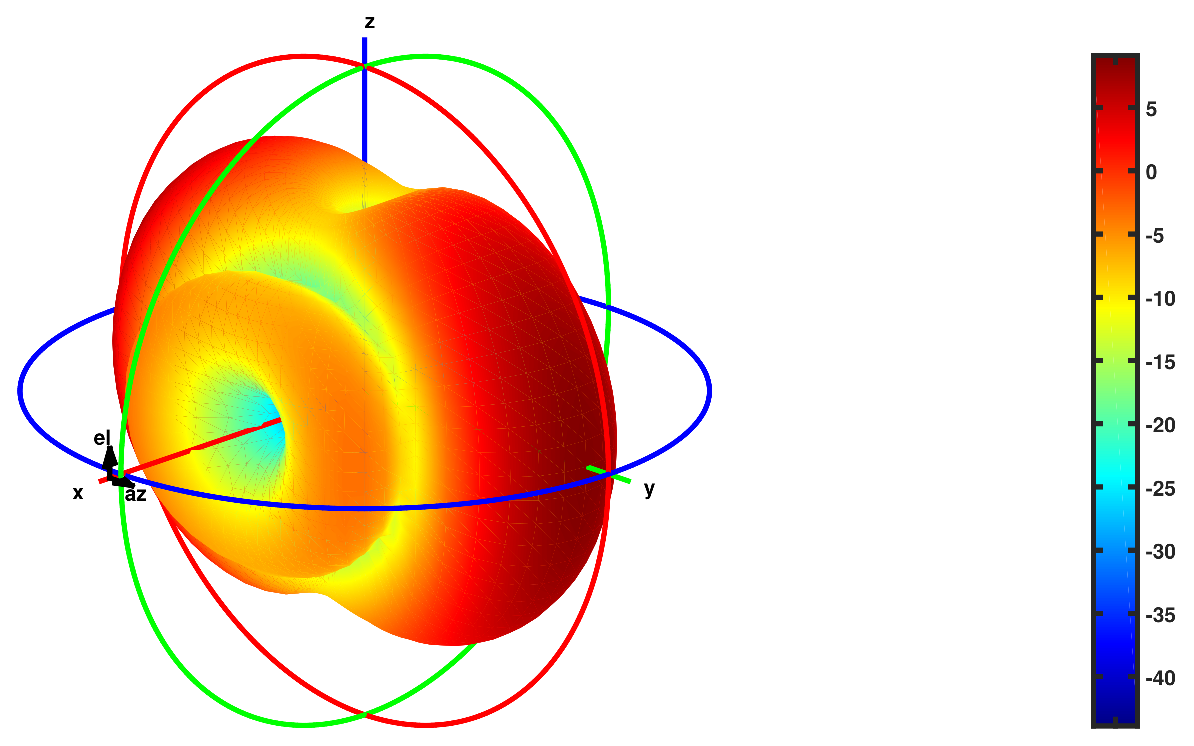
\includegraphics[width=0.46\textwidth]{images/Gill/5G/n_4_9_23.eps}}\hspace{1mm}
  \subfloat[$N$ = 8]{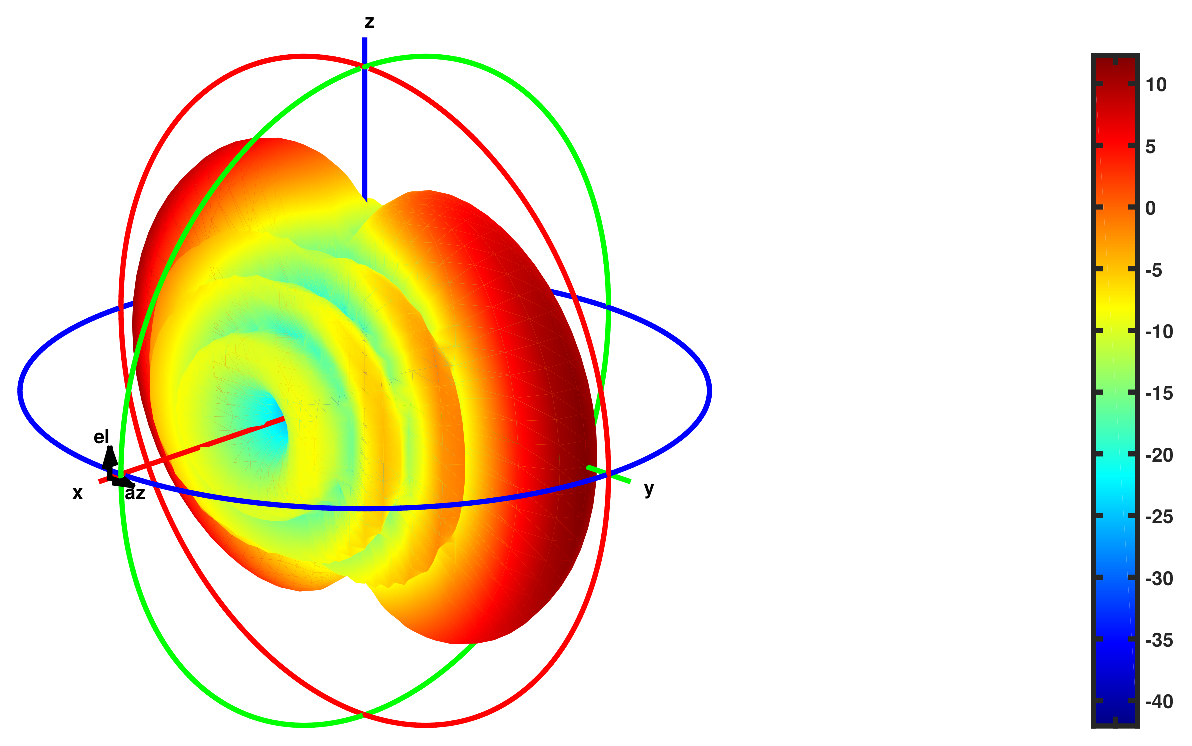
\includegraphics[width=0.46\textwidth]{images/Gill/5G/n_8_12_3.eps}}\hspace{1mm}
  \subfloat[$N$ = 12]{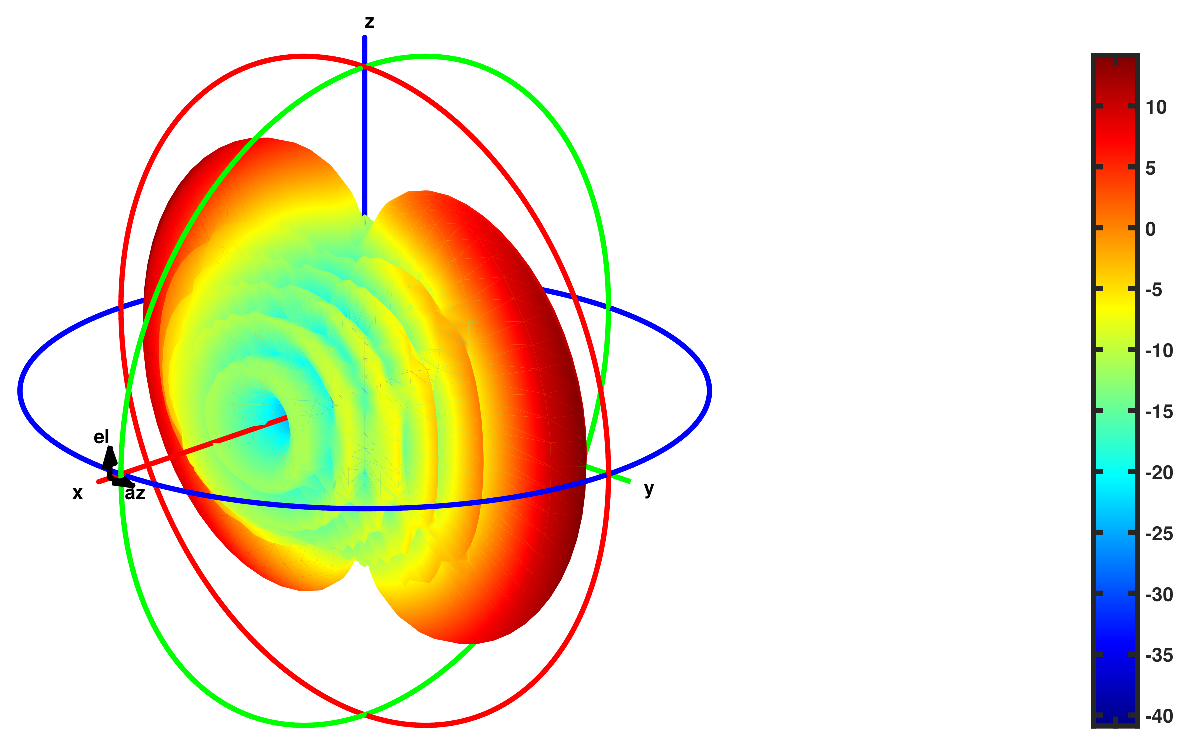
\includegraphics[width=0.46\textwidth]{images/Gill/5G/n_14_1.eps}}\hspace{1mm}
  \subfloat[$N$ = 16]{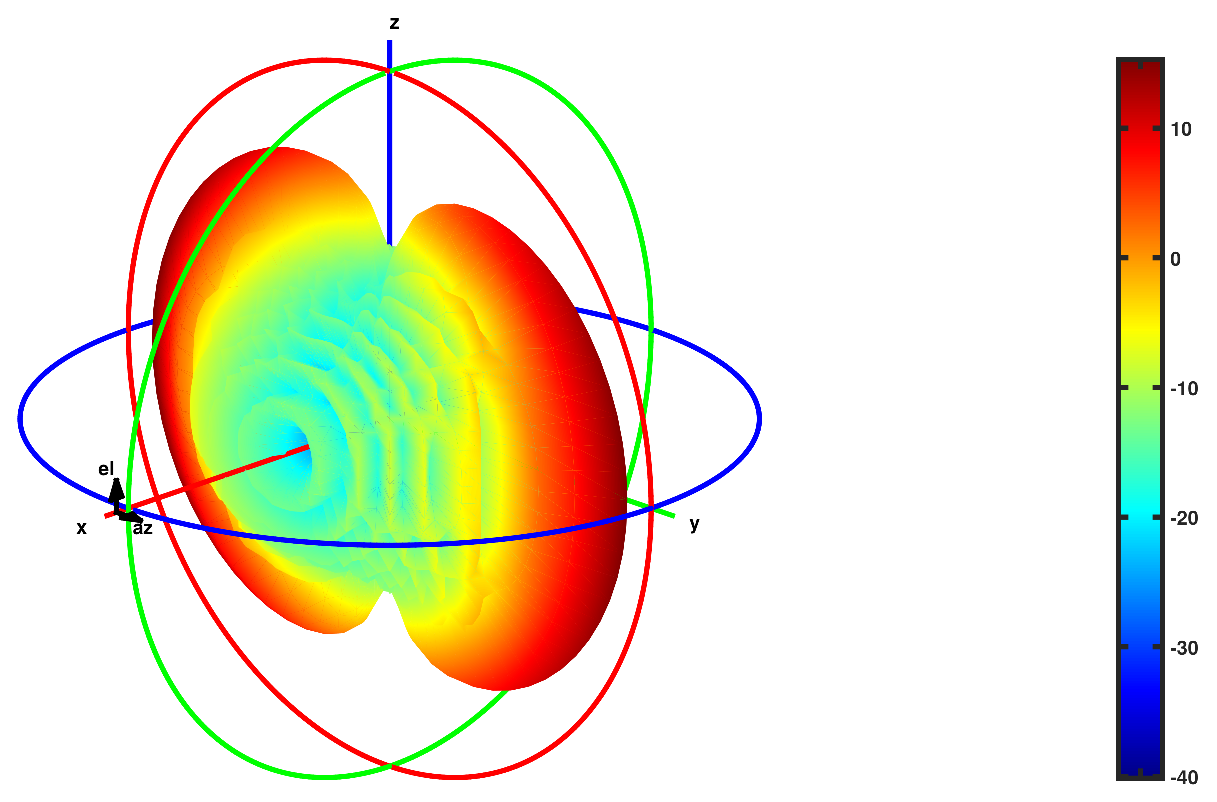
\includegraphics[width=0.46\textwidth]{images/Gill/5G//n_16_15_3.eps}}\hspace{1mm}
  \caption{Beamforming for $N$=4, 8, 12 and 16 linear dipole antenna elements. As the number of antenna element increases we see a sharper beam confined in a smaller region. Massive-MIMO can utilize beamforming to increase spatial gain and spectral efficiency.} 
\label{beamforming}      
\end{figure}

Using Massive-MIMO in 5G system will also lead to making extensive use of inexpensive low-power components, low latency and simplification of media access control (MAC) layer. Although with the arrival of massive-MIMO many traditional problems have become irrelevant, it opens up an entirely new areas research in 5G system. While a very promising technology, massive-MIMO still presents a number of research challenges which need to be addressed. Acquisition of channel state information (CSI) is critical and currently represents the main source of limitations. The mobility of users imposes a finite coherence interval during which channel knowledge must be acquired and utilized, and consequently there is a finite number of orthogonal pilot sequences that can be assigned to the devices~\cite{Boccardi2014}. There is still a lot of research which need to be conducted in massive-MIMO propagation, some experiments thus far have supported the hypothesis of channels being quasi-orthogonal. Synchronization is also very important issue for large number of antenna arrays with the need for reduced power consumption. These are some of the issues which need to be taken care of, for the next generation cellular system.

From above discussion, it can be concluded that implementation of massive-MIMO for 5G cellular system could represent an important breakthrough and major leap with respect to the current state-of-the-art in cellular technology. These modifications at system level needs to be justified for its massive infrastructure cost by solving the challenges currently faced by this key technology via simulations and test-bed experimentations.

\subsection{Machine-to-Machine (M2M) Communication}

Machine to machine (M2M) communication is a new paradigm proposed to be a key technology in 5G wireless systems that enables the ubiquitous connectivity  between a set  of devices  with different network stack.  Thus,  the  autonomous  connection  of  devices  facilitates  the  emergence  of  a  wide  range  of  intelligent M2M applications. M2M exhibits a strong potential to improve human life in different fields such as e-Health, smart  grids, smart cities, intelligent transportation and surveillance enabling internet of things (IoT) applications. A native inclusion of M2M communication in 5G involves satisfying three fundamentally different requirements associated with different classes of low data rates and power consumption services such as: enabling massive number of low-rate devices simultaneously, a minimal data rate in virtually all scenarios, even in worst fading environment and finally managing the above two requirements with a very low latency.


\begin{figure}[!ht]
	\centering
\includegraphics[width=\textwidth,keepaspectratio]{images/Gill/5G/device2device.eps}
	\caption{Machine-to-Machine communication paradigm in 5G Cellular System.}
	\label{d2d}
\end{figure}

Implementing these requirements for 5G system, new communication paradigms needs to be developed at network and physical layer. Figure~\ref{d2d} shows the machine-to-machine communication and how it helps in integrating devices which can be used in health care, localization, vehicular communication, remote maintenance and consumer electronics. In the future standardization of the  5G  networks, the M2M communication is  recognized as one of the key technologies that will support the 5G architecture. As a consequence of this proliferation of M2M technology, large numbers of devices will produce huge amount of irregular data and significantly higher capacity of cellular networks will be needed, in terms of spectrum, power control as well as the number of devices serviced simultaneously. For next generation 5G system, it would be common to have situations where devices will be in close proximity to each other and would like to wirelessly share data like videos, images, etc. or would like to interact for gaming, social networking. If these communication scenarios are handled by simply connecting through the network it can lead to various inefficiencies at various levels. The reason is that cellular networks were primarily designed to support mobile devices with a large amount of data to transmit, whereas most M2M  communications are duty-cycling and  delay-tolerant with small data packets between stationary terminals~\cite{laya2014random}. Thus,  connecting a massive  number  of  M2M  devices  directly  with  cellular networks will saturate uplink traffic easily~\cite{chen2014survey}. In this context, non-cellular connections should serve as important supplement and extension to cellular networks. Some of the challenges of connecting the devices via cellular networks are:

\begin{itemize}
\item Multi-hopping is used to reach destination which otherwise requires fundamentally a single hop. This entails a multi-fold waste of signaling resources as well as higher latency.

\item Huge amount of transmit power is consumed in uplink( fraction of a watt) and downlink( several watts) for data communication which can be easily achieved by milli-watts of power. This leads to unnecessary levels of battery drainage and interference to all other devices occupying the same signaling resources in near proximity.

\item Propagation path-losses to the base stations are much stronger than direct link to the device, hence the corresponding spectral inefficiencies are also lower.
\end{itemize}

It is pretty evident that M2M has huge potential to handle single hop inter device communication more efficiently but these task could be offloaded to other radio access technologies such as Bluetooth, ultra-wide band (UWB) or Zigbee. The applications requiring a mixture of low-latency and high data rates for e.g. interaction between users via augmented reality could be more apt for 5G M2M communication system. In particular, machine-to-machine is as an important enabler for applications requiring low latency, especially in future network deployments utilizing baseband centralization and radio virtualization. There are still various research challenges which need to be taken care of before we can integrate this technology in 5G cellular communication system. The devices for M2M communication need to be designed from both hardware and protocol perspective by providing the needed flexibility at both the PHY and MAC layers. Research needs to be conducted for possible extra overheads for control and channel estimation and also accessing of true net gains associated with M2M mode. And finally, accurate simulation and experimental test-beds needs to be designed for testing M2M communication.

\subsection{Spectrum Regulation for 5G}

Departing from technical issues, we now discuss the crucial interactions that 5G will encounter with spectrum policy and allocation by the federal communications commission (FCC). As already discussed in Section~\ref{5gcell} the spectrum allocated for cellular technologies is already saturated in peak markets due to massive amounts of wireless services and networks. Figure~\ref{specalloc} shows the pronounced scarcity in the the wireless cellular bands as seen in the FCC frequency allocation chart. Large amount of unused spectrum is available in the mm-Wave realm and can be used for high data rate applications. Due to different propagation characteristics for signals at low and sub-terahertz frequencies, future systems will need to integrate a broad range of frequencies. Frequencies on a lower spectrum can be used for wide coverage, mobility support, control signaling and high frequencies for high data rate applications in small cells. This requires a new approach to spectrum policy and allocation methods for 5G standardization.

\begin{figure}[!ht]
	\centering
\includegraphics[width=\textwidth,keepaspectratio]{images/Gill/5G/specalloc.eps}
	\caption{Machine-to-Machine communication paradigm in 5G Cellular System.}
	\label{specalloc}
\end{figure}

Cognitive radio is a promising technology that can solve the spectrum shortage problem arising due to the rapid increase in wireless networks and mobile devices. Recent advancements in software-defined radio technology and edge computing have enhanced the cognitive radio network (CRN)  capabilities and, along with some adjustments in its operation, will be a key technology for 5G heterogeneous network deployment.  The CR network is an innovative software-defined radio technique considered to be one of the key technologies to improve the utilization of the congested radio spectrum~\cite{rusek2013scaling}. Integrating CR technology into 5G system is motivated by the fact that a large portion of the radio spectrum is underutilized most of the time. For achieving data rates in order of gigabits per second, we need to make an efficient use of available spectrum which can be achieved by utilizing CRNs. In CR networks, a secondary system can share spectrum bands with the incumbent primary system, either on an interference-free basis or on an interference-tolerant basis. The CR network should be aware of
the surrounding radio environment and regulate its transmission accordingly. In interference-free CR networks, CR users are allowed to borrow spectrum resources only when licensed users do
not use them. A key to enabling interference-free CR networks is figuring out how to detect the spectrum holes (white space) that spread out in wideband frequency spectrums and facilitate dynamic spectrum access (DSA) smoothly~\cite{wyglinski2009cognitive}. 

CR receivers should first monitor and allocate the unused spectrum via spectrum sensing (energy detection (ED), covariance absolute value (CAV) detection, etc.) or combining with geolocation databases and feed this information back to the central CR controller. A coordinating mechanism is required in multiple CR networks that try to access the same spectrum to prevent users colliding when accessing the matching spectrum holes. In interference-tolerant CR networks, CR users can share the spectrum resource with a licensed system while keeping the interference below a threshold. In comparison with interference-free CR networks, interference-tolerant CR networks can achieve enhanced spectrum utilization by opportunistically sharing the radio spectrum resources with licensed users, as well as better spectral and energy efficiency. However, it has been shown that the performance of CR systems can be very sensitive to any slight change in user densities, interference threshold, and transmission behaviors of the licensed system. However, the spectral efficiency can be improved by either relaxing the interference threshold of the primary system or considering only the CR users who have short distances to the secondary BS (utilizing the spatial gain). Hybrid CR networks have been proposed in~\cite{hong2010capacity} for adoption in cellular networks to explore additional bands and expand the capacity. CR networks can only prove beneficial if the spectrum policies related to 5G are implemented in a robust manner. 



\section{5G using Millimeter Wave (mmWave)}

The massive growth in wireless traffic has drawn an increased attention to the large amount of underutilized spectrum in the mm-Wave frequency bands as a possible solution for achieving gigabits of speed as promised for 5G implementation. Current spectrum for cellular radio (under 5 GHz) is congested and using CR network it can be made more efficient, but for 5G cellular system it is still better to go for bands above 10 GHz. A vast amount of largely unused spectrum is available and can be utilized for 5G. Wireless community has earlier ruled out mm-Wave for cellular usage due to the high penetration loss and its limited usage for short-range communications. And there was also the concern that rain and atmosphere make mm-Wave spectrum useless for mobile communications. The former problem is solved by dividing the cellular architecture into outdoor and indoor environment so that high-data rate applications can be implemented for direct line-of-sight (LOS) communication. As for latter when one considers the fact that today’s cell sizes in urban environments are on the order of 200 m, it becomes clear that mm-wave cellular can overcome these issues~\cite{6515173}. In~\cite{roh2014millimeter} recent results from channel measurement campaigns and development of advanced algorithms, a prototype is discussed in details which makes mm-Wave band a worthy candidate for next generation 5G cellular system.

\begin{figure}[!ht]
	\centering
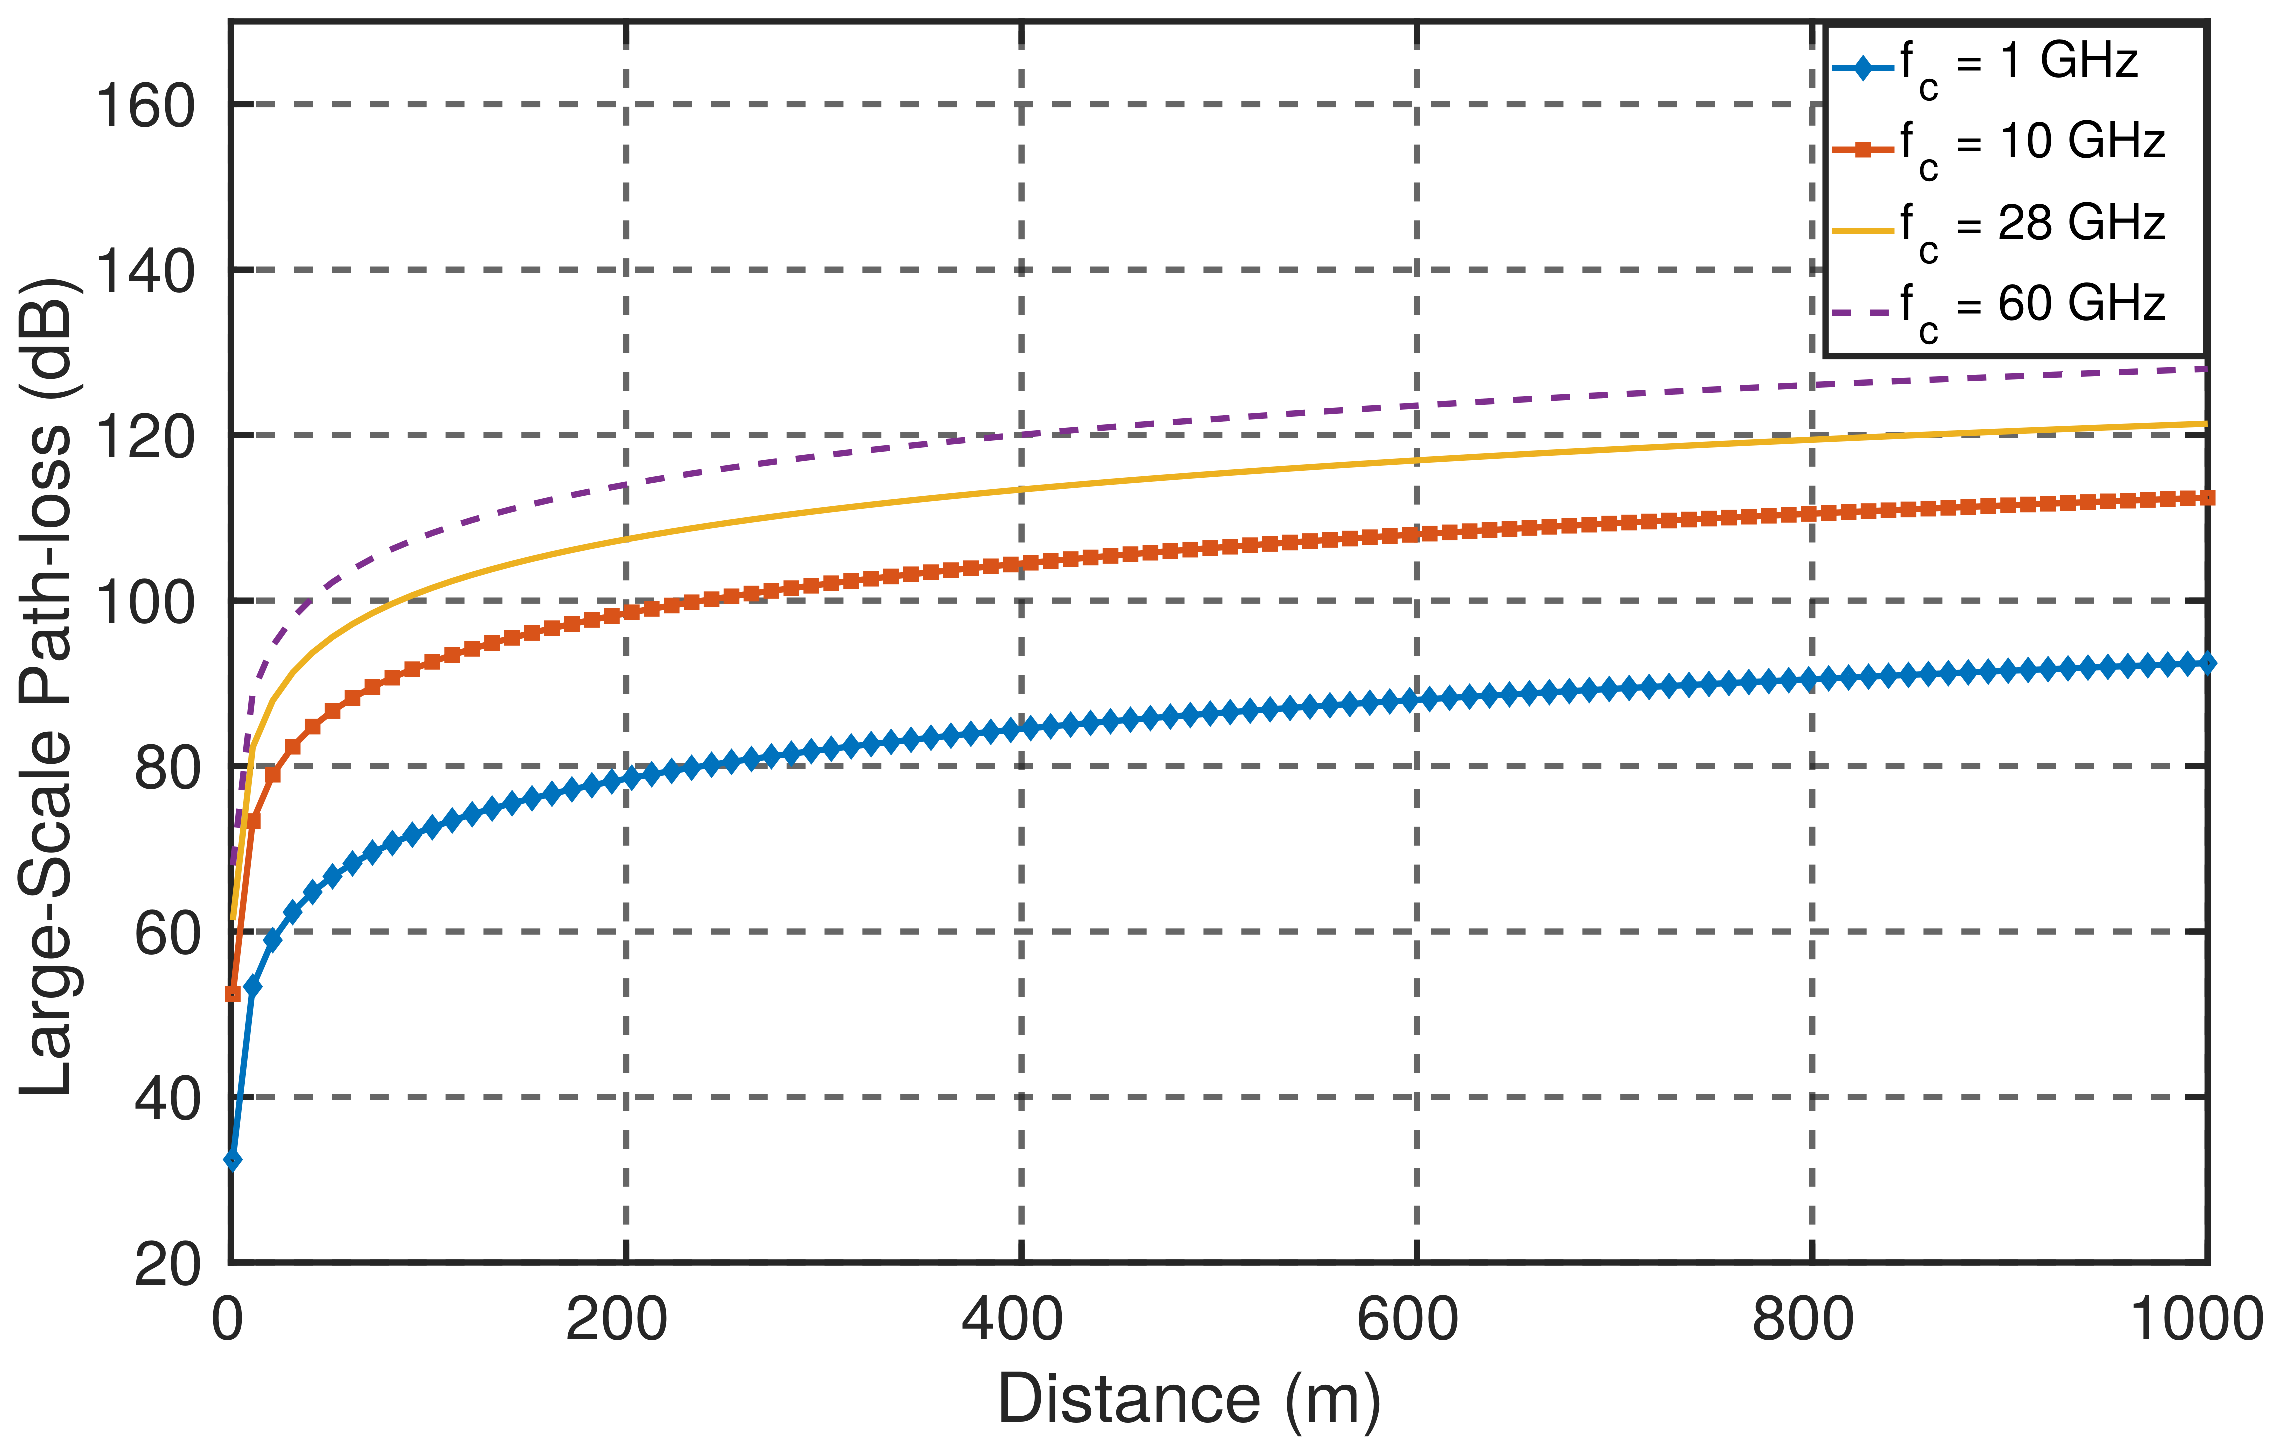
\includegraphics[width=\textwidth,keepaspectratio]{images/Gill/5G/pathloss.eps}
	\caption{Large-scale propagation loss for $f_c$ = 1 GHz, 10 GHz, 28 Ghz and 60 GHz.}
	\label{pathloss}
\end{figure}

Concerns regarding the propagation characteristics at higher frequencies such as higher penetration, precipitation, and foliage losses are legitimate even though the actual amounts of additional propagation losses vary depending on the material of the building, the strength of rain, or the thickness of foliage. Figure~\ref{pathloss} shows the large-scale propagation loss for different frequencies and as we can see that as we go higher in frequencies, path-loss increases for an isotropic antenna. The plot also shows that after certain distance the propagation losses almost saturates and doesn't deteriorate as sharply as they do in first 10 meters. The most common misunderstanding, however, of the propagation characteristics at higher frequencies is that they always incur a much higher propagation loss even in free space compared to lower frequencies, and thus are not adequate for long-range communications. In~\cite{6515173} they have conducted laboratory measurements using a patch antenna at 3 GHz and an array antenna at 30 GHz of the same physical size within an anechoic chamber. And their results shows same amount of propagation loss regardless of the operating frequency when an array antenna of the same physical aperture size is used at the 30 GHz receiving end. And additionally they also showed when array antennas are used at both transmitting and receiving ends at 30 GHz, the measured receive power is 20 dB higher than that of the 3 GHz patch antenna case. To understand how the path-loss is same for 3 GHz and 30 GHz frequencies let's start with friis equation.
\begin{equation}
\label{eqfriis}
P_r = P_t+G_t+G_r+20\log\bigg(\dfrac{c}{4\pi df}\bigg)
\end{equation}
where $P_r$ is the received power in free space, $P_t$ is the transmit power, $G_t$, $G_r$ are transmit and receive antenna gains, respectively, $d$ is the distance between the transmitter and receiver in meters, $f$ is the carrier frequency and $c$ is the speed of light. From Eq.(\ref{eqfriis}) it is pretty evident that received power is inversely proportional to the frequency squared for an ideal isotropic antenna. However, in reality antennas or an antenna arrays have gains of $G_t$ and $G_r$ greater than 1 and are typically employed at both ends. The most important factor for advocating mm-Wave is that antenna gains are proportional to the frequency squared given a fixed physical aperture size~\cite{friis1946note}. Given the same physical aperture size, therefore, transmit and receive antennas at higher frequencies, in fact, send and receive more energy through narrower directed beams, which is not commonly recognized. And since he physical size of antennas at mm-Wave frequencies is so small that it becomes practical to build hundreds and thousands of antennas elements to provide huge gains from spatial isolation and multiplexing for 5G cellular communication system.

\section{Vehicular Communication Using 5G}
With the development of mm-Wave and massive-MIMO, the spectral and energy efficiency for 5G wireless communications has been drastically improved. The development of driverless cars has posed some rigorous requirements for the safety of the passengers and pedestrians. For safety-critical applications the transmission delay needs to be less than 1 ms which is required for intelligent transportation systems (ITSs) and vehicular networks~\cite{ge2016vehicular}. Considering the drawbacks of IEEE 802.11p networks, such as poor scalability, low capacity , and intermittent connectivity, the Long Term Evolution (LTE) mobile communication technologies were proposed to support vehicular applications~\cite{araniti2013lte}. Simulation and experiment results revealed that there is a trade-off between the proposed performance metrics and system parameters, such as base station (BS) and vehicle densities, radio coverage, and  the  maximum  number of hops in a path. When LTE communication technologies have been integrated into vehicular networks, the interference has cut down the performance of LTE vehicular networks. When vehicle density is high, the beaconing signals of vehicular safety applications may easily overload the serving eNodeB. To handle this issue, a significant amount of such signals should be distributed directly among vehicles, without  going  through  the  eNB. In  LTE-Advanced (LTE-A), device-to-device (D2D) communication is considered to allow direct message delivery between terminals in proximity to lighten the load of eNB~\cite{mumtaz2014direct}. 

\begin{figure}[!ht]
	\centering
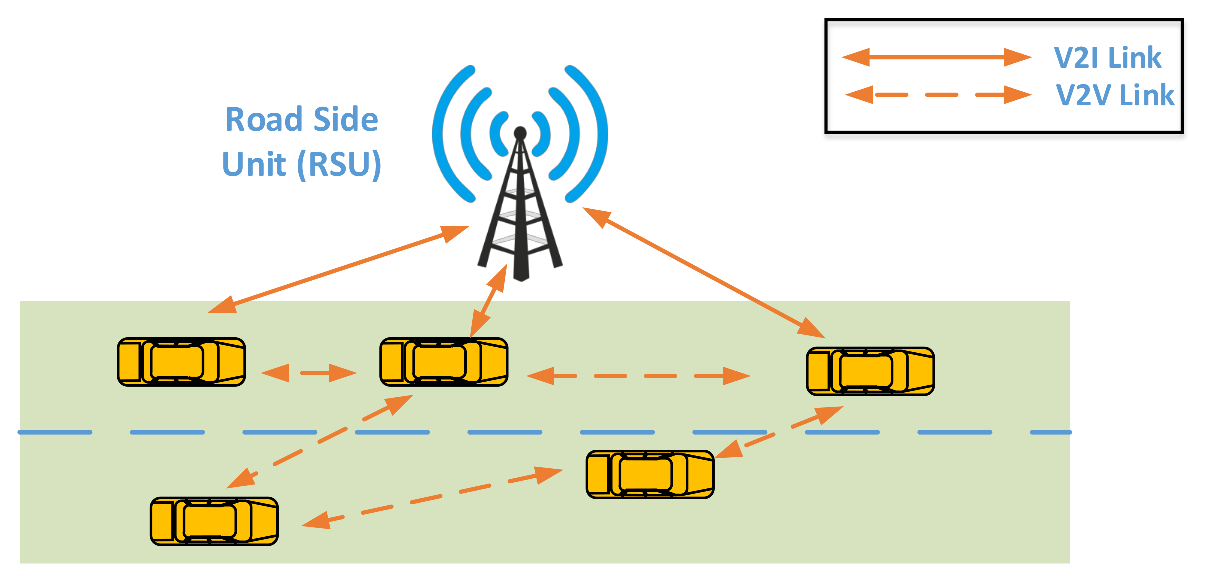
\includegraphics[width=\textwidth,keepaspectratio]{images/Gill/5G/vehiclecomm.eps}
	\caption{Vehicular communication using D2D 5G cellular communication technology.}
	\label{vcomm}
\end{figure}

Hence the infrastructure-aided D2D technologies can serve as a natural approach to enable reliable and efficient V2V communications without negatively affecting existing cellular systems. To meet the high performance requirements, such as low transmission delay and high throughput, a new architecture for 5G vehicular communication is required. Figure~\ref{vcomm} describes the vehicular communication  using D2D communication strategy where significant amount of computation is offloaded from road side units (RSU) to vehicles to avoid increase spectral and efficiency. The communication environment in V2V is quite different than in D2D due to high mobility (Doppler shift) of vehicles. Network connectivity play a important role in V2V communication than D2D, compared with system throughput. These features can significantly affect D2D resource allocation strategies and system parameters, and thus should be modified for vehicular communication.

\section{Summary}
\textbf{Summary will go here for now use this demo msg} CR receivers should first monitor and allocate the unused spectrum via spectrum sensing (energy detection (ED), covariance absolute value (CAV) detection, etc.) or combining with geolocation databases and feed this information back to the central CR controller. A coordinating mechanism is required in multiple CR networks that try to access the same spectrum to prevent users colliding when accessing the matching spectrum holes. In interference-tolerant CR networks, CR users can share the spectrum resource with a licensed system while keeping the interference below a threshold. In comparison with interference-free CR networks, interference-tolerant CR networks can achieve enhanced spectrum utilization by opportunistically sharing the radio spectrum resources with licensed users, as well as better spectral and energy efficiency. However, it has been shown that the performance of CR systems can be very sensitive to any slight change in user densities, interference threshold, and transmission behaviors of the licensed system. However, the spectral efficiency can be improved by either relaxing the interference threshold of the primary system or considering only the CR users who have short distances to the secondary BS (utilizing the spatial gain). Hybrid CR networks have been proposed in~\cite{hong2010capacity} for adoption in cellular networks to explore additional bands and expand the capacity.


